\documentclass[a4paper, 12 pt]{article}
\usepackage[utf8]{inputenc}
\usepackage[T1]{fontenc}
\usepackage[slovene]{babel}
\usepackage{lmodern}
\usepackage{amsmath}
\usepackage{amsfonts}
\usepackage{amssymb}
\usepackage{units}
\usepackage{eurosym}
\usepackage{pdfpages}
\usepackage{comment}
\usepackage{enumerate}
\usepackage{mathtools}
\usepackage{amsthm}
\usepackage{float}


% Matematicna okolja
\theoremstyle{definition}
\newtheorem*{definicija}{Definicija}
\newtheorem*{primer}{Primer}

\theoremstyle{plain}
\newtheorem*{lema}{Lema}
\newtheorem*{izrek}{Izrek}
\newtheorem*{trditev}{Trditev}
\newtheorem*{posledica}{Posledica}

\theoremstyle{remark}
\newtheorem*{opomba}{Opomba}


% ==============================================================
\begin{document}
\begin{titlepage}
		\begin{center}
		
		\large
		Univerza v Ljubljani\\
		\normalsize
		Fakulteta za matematiko in fiziko\\
		
		\small
		Finančna matematika - 1. stopnja\\
		
		\vspace{5 cm} 
		
		\large
		Matej Škerlep \\
		
		\vspace{0.5cm}
		\LARGE
		\textbf{Problem največje neodvisne množice}
		
		\vspace{0.5 cm}
		\normalsize
		Projekt pri predmetu finančni praktikum
		
		\vspace{1.5cm}
		\normalsize
		Mentorja: prof. dr. Riste Škrekovski in asist. dr. Janoš Vidali
		
		\vfill
		
		\large Ljubljana, 2020
		
		\end{center}
\end{titlepage}
% ==========================================================
\tableofcontents

\listoffigures

\newpage
\listoftables
\newpage
% ==========================================================
\section{Predstavitev problema} % ============================================

\subsection{Navodila za delo}

Definirajte problem največje množice nesosednjih vozlišč kot CLP in ga rešite za nekaj primerov. Eksperimentalno primerjajte rezultate CLP in njegove relaksacije na LP in ugotovite, za koliko se lahko razlikujejo med sabo po velikosti. Napišite algoritem za lokalno iskanje po grafu in njegov rezultate primerjajte s prejšnjimi. Ugotovite za kako velike grafe je posamezen izmed primerov rešljiv.

%\begin{itemize}
%\item Definirajte problem največje množice nesosednjih vozlišč kot CLP in ga rešite za nekaj primerov. 
%\item Eksperimentalno primerjajte rezultate CLP in njegove relaksacije na LP in ugotovite, za koliko se lahko razlikujejo med sabo po velikosti.
%\item Napišite algoritem za lokalno iskanje po grafu in njegov rezultate primerjajte s prejšnjimi. 
%\item Ugotovite za kako velike grafe je posamezen izmed primerov rešljiv.
%\end{itemize}

\subsection{Definicije pojmov}

\begin{definicija}Naj bo $G = (V, E)$ graf in $I \subseteq V$. Množica vozlišč $I$ je \textbf{\textit{neodvisna}}, če ne vsebuje sosednjih vozlišč. 
\newline Formalno, če za $\forall v, u \in V$, $uv \in E$ velja $v \in I \Leftrightarrow  u \notin I$.
\end{definicija}

\begin{primer}
Oglejmo si preprost primer največje neodvisne množice na grafu s 7 vozlišči. Množica vozlišč $\{3, 4, 5, 6\}$ predstavlja največjo množico neodvisnih vozlišč.
\begin{figure}[H]
\centering
  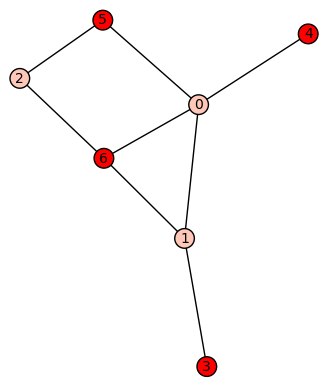
\includegraphics[scale=0.4]{./Slike/neodvisna_zgled.png}
  \caption{Primer največje neodvisne množice na grafu s sedmimi vozlišči}
  \label{fig:primer7vozlisc} 
\end{figure}
\end{primer}

\subsection{Celoštevilski linearen program}
Tako kot zgoraj v definiciji, bo v celotni nalogi največja neodvisna množica označevana z $I$. Za začetek si oglejmo celoštevilski linearen program za opisani problem.  Vsakemu vozlišču $v \in V$ priredimo spremenljivko $x_v$ z vrednostmi 0 ali 1. Pri tem je 
\[   
x_v = 
     \begin{cases}
       1; &v \in I \\
       0; &v \notin I\\
     \end{cases}
\]
Pogoj $x_u + x_v \leq 1, \ \forall uv \in E$ nam tako zagotovalja, da ima vsaka povezava $uv \in E$ največ eno vozlišče v množici $I$. Vrednost kriterijske funkcije spodnjega CLP je enaka moči množice $I$, v njej pa so vsa vozlišča $v$ za katera je $x_v = 1$.

\begin{equation*}
\begin{array}{ll@{}ll}
\text{max}  & \displaystyle\sum\limits_{v\in V} x_v &&\\
\text{p.p.}	 & x_u + x_v \leq 1,		 			&&\text{za vsak par } uv \in E \\
                 & x_v \in \{0,1\}, 	              			&&\forall v \in V
\end{array}
\end{equation*}




\subsection{Relaksacija celoštevilskega linearnega programa} \label{RCLP}
V primeru relaksacije LP pogoj $x_v \in \{0, 1\}$ zamenjamo s pogojem\\ $0 \leq x_v \leq 1$:

\begin{equation*}
\begin{array}{ll@{}ll}
\text{max}  	& \displaystyle\sum\limits_{v\in V} x_v &&\\
\text{p.p.}	& x_u + x_v \leq 1,		 				&&\forall uv \in E \\
                 	& 0 \leq x_v \leq 1, 	              	&&\forall v \in V.
\end{array}
\end{equation*}

V tem primeru dobimo trivialno rešitev $x_v = \frac{1}{2}$ za $\forall v \in V$, ki pa nam o tem katera vozlišča so v množici $I$ ne pove ničesar. Zato bomo v množico $I$ dodajali zgolj tista vozlišča, ki bodo imela vrednost $x_v > \frac{1}{2}$. S tem zagotovimo, da bo v $I$ nastopalo največ eno vozlišče vsake povezave, s čemer bomo dobili neodvisno množico in torej dopustno rešitev. V nadaljevanju bomo videli, da se pogosto zgodi, da je prav rešitev $x_v = \frac{1}{2}$ za $\forall v \in V$ optimalna in posledično (glede na pogoj $x_v \in I \iff x_v > \frac{1}{2}$) bo množica $I$ prazna.
%V primeru relaksacije LP je torej vrednost kriterijske funkcije nazdol omejena z optimalno vrednostjo.
 
\newpage
\section{Algoritmi} % ===================================================
\subsection{Izbira programskega jezika in knjižnic}
Algoritmi so napisani v programskem jeziku \textit{Sage}, ki temelji na programskem jeziku \textit{Python}. Uporabil sem module \textit{time} za merjenje časa za izvedbo posameznega algoritma, \textit{random} za generiranje naključnega nabor vozlišč v algoritmu lokalnega iskanja in \textit{csv} za shranjevanje rezulatov poskusov v csv obliki.

V kodi sem najprej napisal vse tri funkcije \verb|clp|, \verb|rclp| in \verb|lokalno_iskanje|. Nato sem za namen testiranj napisal funkcijo \verb|testiraj|, ki na naključnem grafu (kot argumente grafa določimo število vozlišč in verjetnost povezave med dvema vozliščema) izvede vse tri zgoraj omenjene funkcije in kot rezultat vrne seznam izhodnih podatkov vseh treh funkcij. Na koncu pa je še funkcija \verb|izpis_csv|, ki rezultate testiranj zapiše v csv datoteteko. Posamezna vrstica v csv datoteki predstavlja izhodne podatke vseh treh algoritmov za graf na določenem številu vozlišč. Teste sem na koncu izvedel še na Petersenovem grafu in na hiperkockah.

Za namene analize časovne zahtevnosti, so v vseh treh funkcijah uporabljeni klici \verb|time.time()|, čas celotne izvedbe posameznega algoritma pa nato dobimo kot razliko med končnim in začetnim časom (t.j. \verb|cas = kon - zac|).

\subsection{Celoštevilski linearni program} \label{CLP}
\begin{verbatim}
def clp(graf):
    zac = time.time()

    CLP = MixedIntegerLinearProgram(maximization = True) 
    vozlisca = CLP.new_variable(binary = True) 
    CLP.set_objective(sum([vozlisca[v] for v in graf.vertices()])) 
    for u,v in graf.edges(labels = False):
        CLP.add_constraint(vozlisca[u] + vozlisca[v] <= 1) 

    moc_max = CLP.solve() 
    vozlisca = CLP.get_values(vozlisca) 

    sez = [k for k, v in vozlisca.items() if v == 1.0]

    kon = time.time() 
    cas = kon - zac
    return [int(moc_max), sez, cas]
\end{verbatim}
\newpage

Funkcija clp kot vhodni argument vzame nek graf. Celoštevilski linearni program najprej definiramo s funkcijo \verb|MixedIntegerLinearProgram|. Nato za vsako vozlišče priredimo binarno spremenljivko \verb|vozlisca| z vrednostmi 0 ali 1. Kriterijsko funkcijo definiramo s klicem funkcije \verb|set_objective|, omejitev za vsaki dve povezani vozlišči pa z \verb|add_constraint|. Optimalno vrednost kriterijske funkcije dobimo s \verb|CLP.solve()|, kar je hkrati tudi moč največje neodvisne množice. Vrednost $x_v$ posameznega vozlišča pa dobimo z \verb|CLP.get_values(vozlisca)|. V iskano največjo množico neodvisnih vozlišč \verb|sez| torej dodamo vozlišča z vrednostjo $x_v$ enako 1. Kot izhodni podatek na koncu dobimo seznam oblike moc najvecje neodvisne mnozice, seznam vozlisc v tej množici in čas izvedbe algoritma. Funkcija \verb|int()| nam število s plavajočo vejico zapiše v celoštevilski obliki, kar sem uporabil zaradi težav Excela pri branju podatkov.



\subsection{Relaksacija celoštevilskega linearna programa}
\begin{verbatim}
def rclp(graf):
    zac = time.time()

    RCLP = MixedIntegerLinearProgram(maximization = True)
    vozlisca = RCLP.new_variable(real = True)
    RCLP.set_max(vozlisca,1)
    RCLP.set_min(vozlisca,0)
    RCLP.set_objective(sum([vozlisca[v] for v in graf.vertices()]))
    for u,v in graf.edges(labels = False):
        RCLP.add_constraint(vozlisca[u] + vozlisca[v] <= 1)

    RCLP.solve()
    vozlisca = RCLP.get_values(vozlisca)

    sez = [k for k, v in vozlisca.items() if v > 0.5]
    moc_max = len(sez)

    kon = time.time()
    cas = kon - zac
    return [int(moc_max), sez, cas]
\end{verbatim}
Večina komentarjev je podobnih kot pod algoritmom za CLP v razdelku \ref{CLP}, zato bom tu obrazložil le tisto kar se razlikuje. Pri relaksaciji CLP vrednosti $x_v$ omejimo z \verb|set_max| oz. \verb|set_min|. Vrednost kriterijske funkcije nam o moči množice ne pove prav dosti, zato z argumenti iz razdelka \ref{RCLP}, dodajamo v največjo množico neodvisnih vozlišč (v algoritmu označena s \verb|sez|) le tista vozlišča z $x_v > \frac{1}{2}$. Funkcija sprejme in vrne enake argumente kot \verb|clp|.

\subsection{Lokalno iskanje} \label{lokiskalgorit}
\begin{verbatim}
def lokalno_iskanje(graf, st_ponovitev):
    moc_max = 0 
    max_mnozica_neod = set() 
    zac = time.time()
    for i in range(st_ponovitev):
        mnozica_neod = set() 
        mnozica_neod.add(graf.random_vertex()) 
        for v in random.sample(graf.vertices(), len(graf.vertices())):
            if not any(u in mnozica_neod for u in graf[v]): 
                    mnozica_neod.add(v)
        if len(mnozica_neod) > moc_max: 
            max_mnozica_neod = mnozica_neod
            moc_max = len(mnozica_neod)
    kon = time.time()
    cas = kon - zac
    return[moc_max, max_mnozica_neod, cas]
\end{verbatim}

Ideja zgornjega algoritma je sledeča. Začnemo s prazno množico $I$ v katero dodamo naključno izbrano vozlišče. Nato po naključnem naboru vozlišč, v  $I$ dodajamo tista vozlišča, katerih sosedje niso v množici  $I$. To zanko ponovimo poljubno mnogokrat in nato vzamemo tisto  $I$, ki ima največjo moč.


\begin{opomba}
Za razliko od zgornjih dveh algoritmov, kjer sem delal s seznamom, sem pri lokalnem iskanju uporabil množico, saj je s tem zmanjšana časovna zahtevnost algortima (pričakovano konstantna namesto linearne).
\end{opomba}
\newpage
\section{Rezultati} % ===================================================
V namen analize algoritmov sem vse tri zgornje funkcije izvedel na istih naključnih grafih. Kot argumente generiranja grafa sem vzel vse možne kombinacije števila vozlišč (1 do 100) in verjetnosti povezave dveh vozlišč ($\frac{1}{10}, \frac{3}{10}, \frac{5}{10}, \frac{7}{10}$ in $\frac{9}{10}$). Pri tem sem število ponovitev lokalnega iskanja nastavil na 50.

Primerjal sem moči največjih neodvisnih množic vseh treh algoritmov. Podrobnejša analiza je dostopna v datoteki $\textit{analiza\_testov.xlsx}$, tu pa bom opisal predvsem ugotovitve.  Generalno gledano za vse rezultate testiranj velja, da je moč množice dobljene s CLP vedno večja ali enaka moči množice dobljene z lokalnim iskanjem. Algoritem relaksacije CLP od določenega števila vozlišč dalje (pri velikih verjetnostih že od 3 vozlišč naprej), skoraj vedno vrača prazno množico, kar pomeni, da je očitno optimalna vrednost kriterijske funkcije, prav, ko imajo vsa vozlišča vrednost $x_v$ enako $\frac{1}{2}$.

\subsection{Analiza algoritmov na naključnih grafih}

\subsubsection{Primerjava moči množic vseh treh algoritmov}

Za začetek si oglejmo, do katerega števila vozlišč dobimo enake moči dobljenih množic vseh treh algoritmov.



\begin{table}[H]
\centering
\begin{tabular}{|p{2.1cm}|p{3.2cm}|p{6cm}|}
\hline
\textbf{Verjetnost povezave}  & \textbf{Enakost vseh treh algoritmov} \\ \hline
0,1    & do 18 vozlišč   \\ \hline
0,3    & do 7 vozlišč     \\ \hline
0,5    & do 4 vozlišč  \\ \hline
0,7    & do 4 vozlišč \\ \hline
0,9    & do 2 vozlišč    \\ \hline
\end{tabular}
\caption{Enakost moči množice vseh treh algoritmov}
\label{fig:enakost vseh treh} 
\end{table}

Opazno je precejšnje zmanjševanje. Vidimo, da v primeru zelo povezanega grafa, dobimo enakost zgolj še na 2 vozliščih. Glavni razlog za neenakost je relaksacija CLP, za katero je za grafe na večjem številu vozlišč ponavadi optimalna rešitev, ko imajo vsa vozlišča vrednost $\frac{1}{2}$ in posledično moč množice $I$ enaka 0. To je vidno tudi na grafih na straneh \pageref{fig:moc0,1} - \pageref{fig:moc0,9}.

\subsubsection{Primerjava moči množic CLP in lokalnega iskanja}

Bolj zanimivo si je ogledati enakost med močmi množic dobljenih s CLP in lokalnim iskanjem. Spodnja tabela prikazuje do katerega števila vozlišč dobimo enakosti moči in največjo razliko med močema množice $I$ dobljene s CLP in lokalnim iskanjem na vzorcu grafov od 1 do 100 vozlišč pri posamezni verjetnosti.

\begin{table}[H]
\centering
\begin{tabular}{|p{2.1cm}|p{3.7cm}|p{3.5cm}|}
\hline
\textbf{Verjetnost povezave}  & \textbf{Enakost CLP in lokalnega iskanja} & \textbf{Največja razlika v močeh} \\ \hline
0,1    & do 33 vozlišč &  4\\ \hline
0,3    & do 26 vozlišč  &  3   \\ \hline
0,5    & do 35 vozlišč &  2 \\ \hline
0,7    & do 38 vozlišč  &  1\\ \hline
0,9    & do 58 vozlišč  &  1  \\ \hline
\end{tabular}
\caption{Enakost moči množic CLP in lokalnega iskanja ter največje razlike v močeh}
\label{fig:enakost vseh treh} 
\end{table}

Opazimo, lahko, da je najmanjše ujemanje pri nizkih verjetnostih povezave. Enakosti dobivamo do 34 vozlišč, sicer pa je nato do 67 vozlišč razlike v močeh največ 2. Pri grafih z verjetnostjo 0,3 se meja enakosti pomakne nekoliko navzdol, a se hkrati meja, ko je razlike v močeh največ 2, pomakne na 76 vozlišč. Pri višjih verjetnostih se začne meja enakosti precej povečevati, poleg tega pa tudi manjšati maksimalna razlika med močmi dobljenih množic. Pri verjetnosi povezave 0,9 se pojavi le 5 primerov, ko se vrednosti moči razlikujeta za 1, v ostalih primerih pa dobimo enakosti.

\subsubsection{Grafična predstavitev rezultatov}

V namen grafične predstave zgoraj povedanega sem rezultate testiranj prikazal tudi na spodnjih treh grafih, ki nam prikazujejo moči dobljenih množic v odvisnosti od števila vozlišč. Na grafu je prikazana tudi aproksimacija gibanja vrednostni s polinomom šeste stopnje. Kot sem omenil že zgoraj je za večje grafe opazen padec moči množice dobljene s relaksacijo CLP, sploh v primerih z veliko verjetnostjo povezave dveh vozlišč grafa. 
\begin{figure}[H]
\centering
  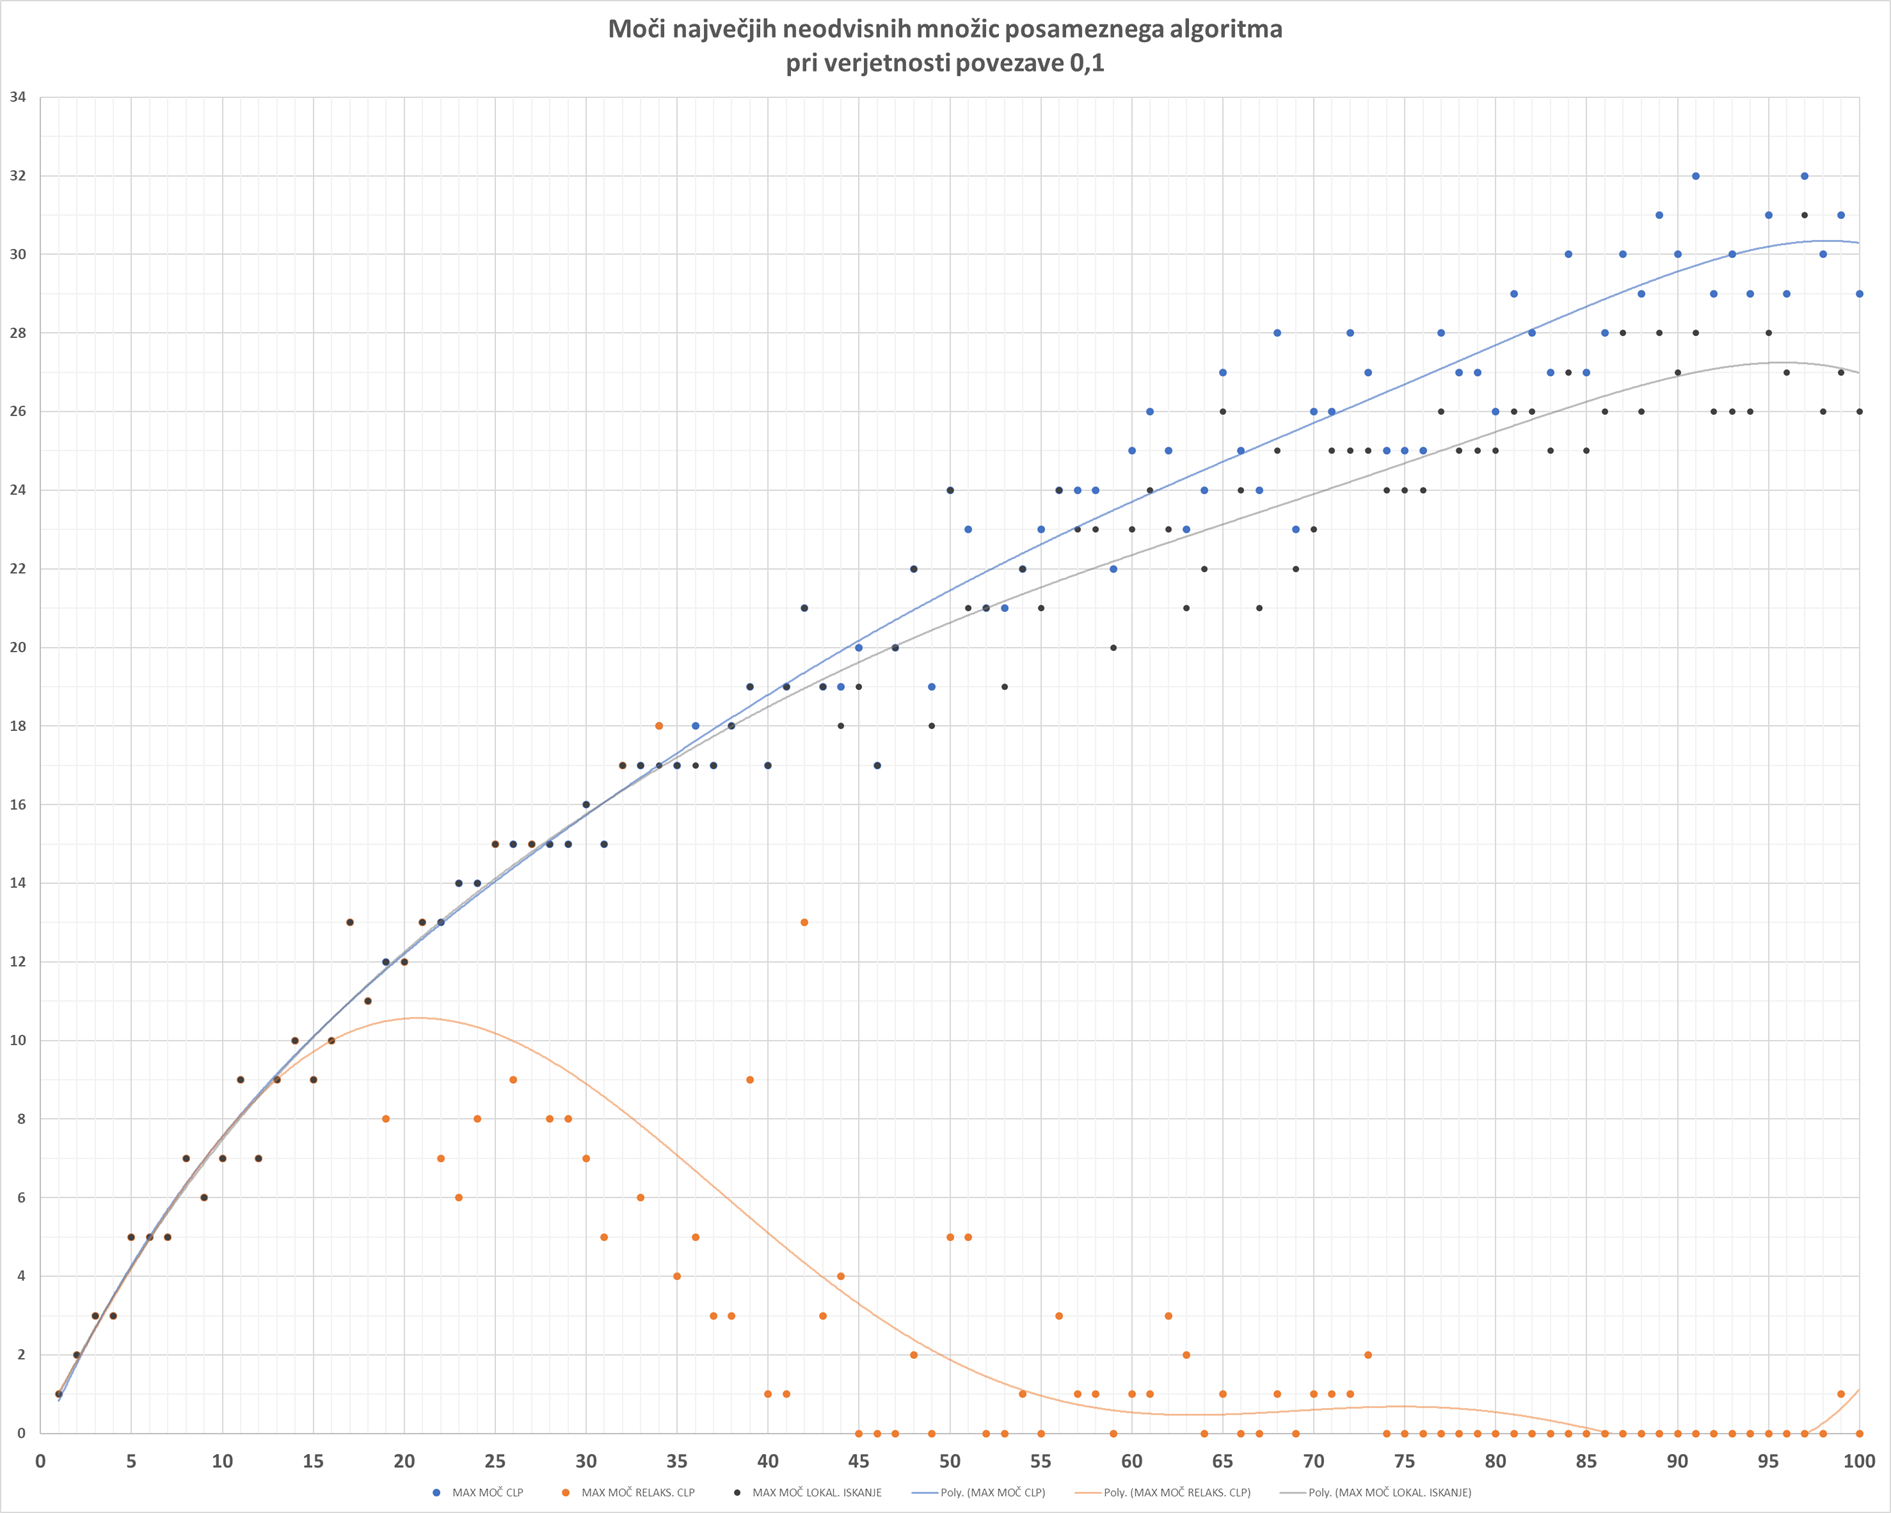
\includegraphics[scale=0.28]{./Slike/0,1 moci.png}
  \caption{Moči največjih neodvisnih množic pri verjetnosti povezave 0,1}
  \label{fig:moc0,1} 
\end{figure}

\begin{figure}[H]
\centering
  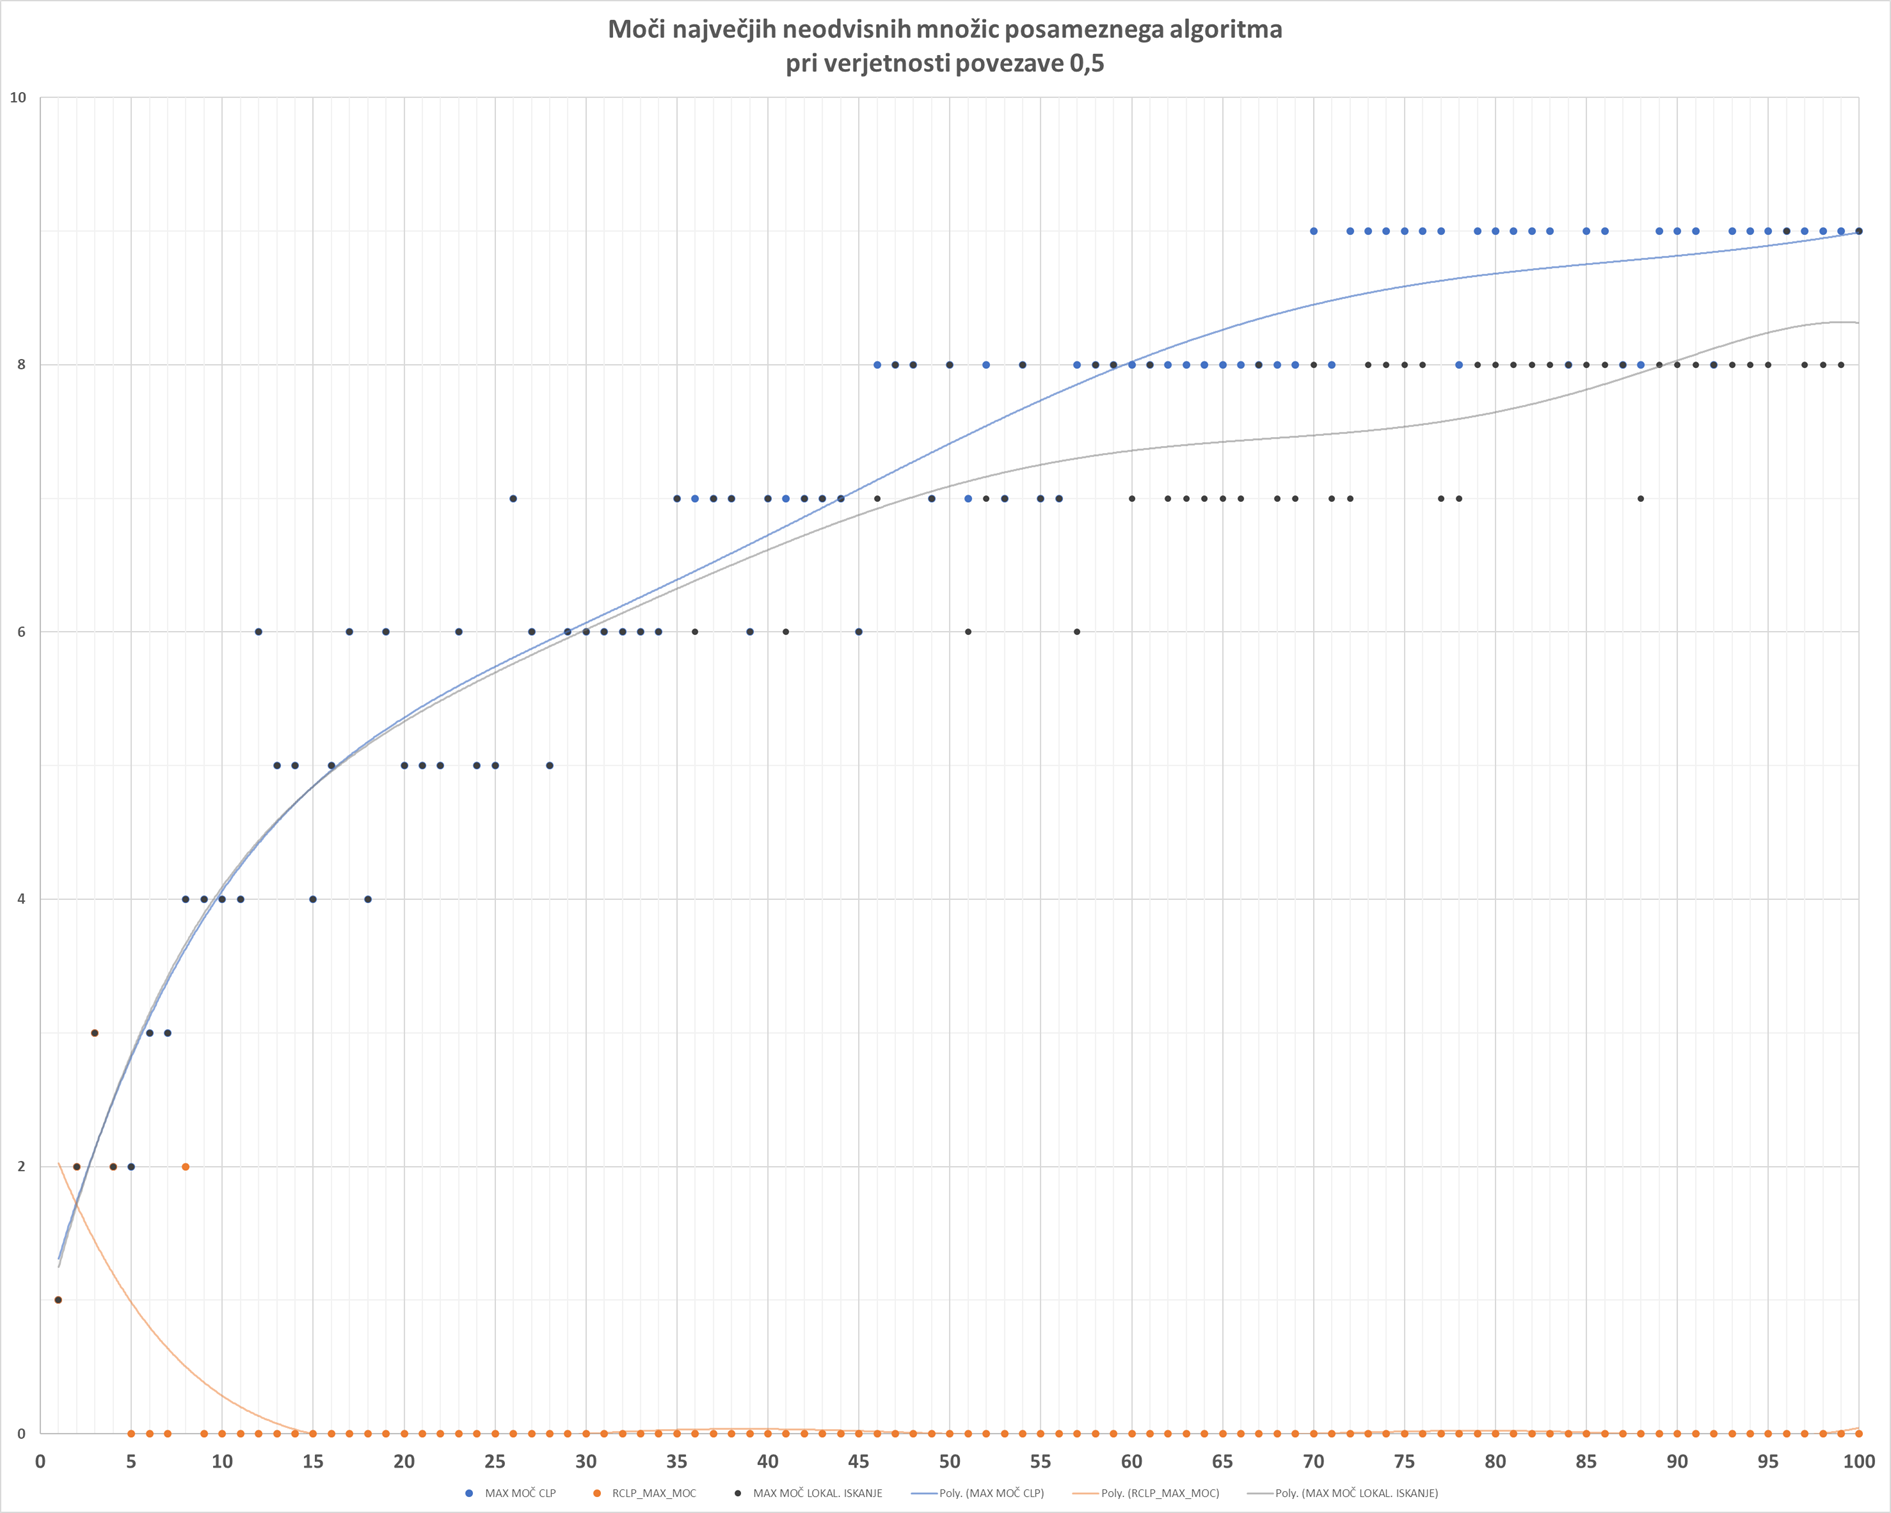
\includegraphics[scale=0.28]{./Slike/0,5 moci.png}
  \caption{Moči največjih neodvisnih množic pri verjetnosti povezave 0,5}
  \label{fig:moc0,5} 
\end{figure}

Zanimivo je, da z večanjem verjetnosti, moč največje neodvisne množice CLP in lokalnega iskanja postaja konstantna na določenih intervalih števila vozlišč. Z večanjem števila vozlišč, se moč množice tudi precej počasneje povečuje in pri zelo povezanih grafih nikoli celo ne preseže vrednosti 5.


\begin{figure}[H]
\centering
  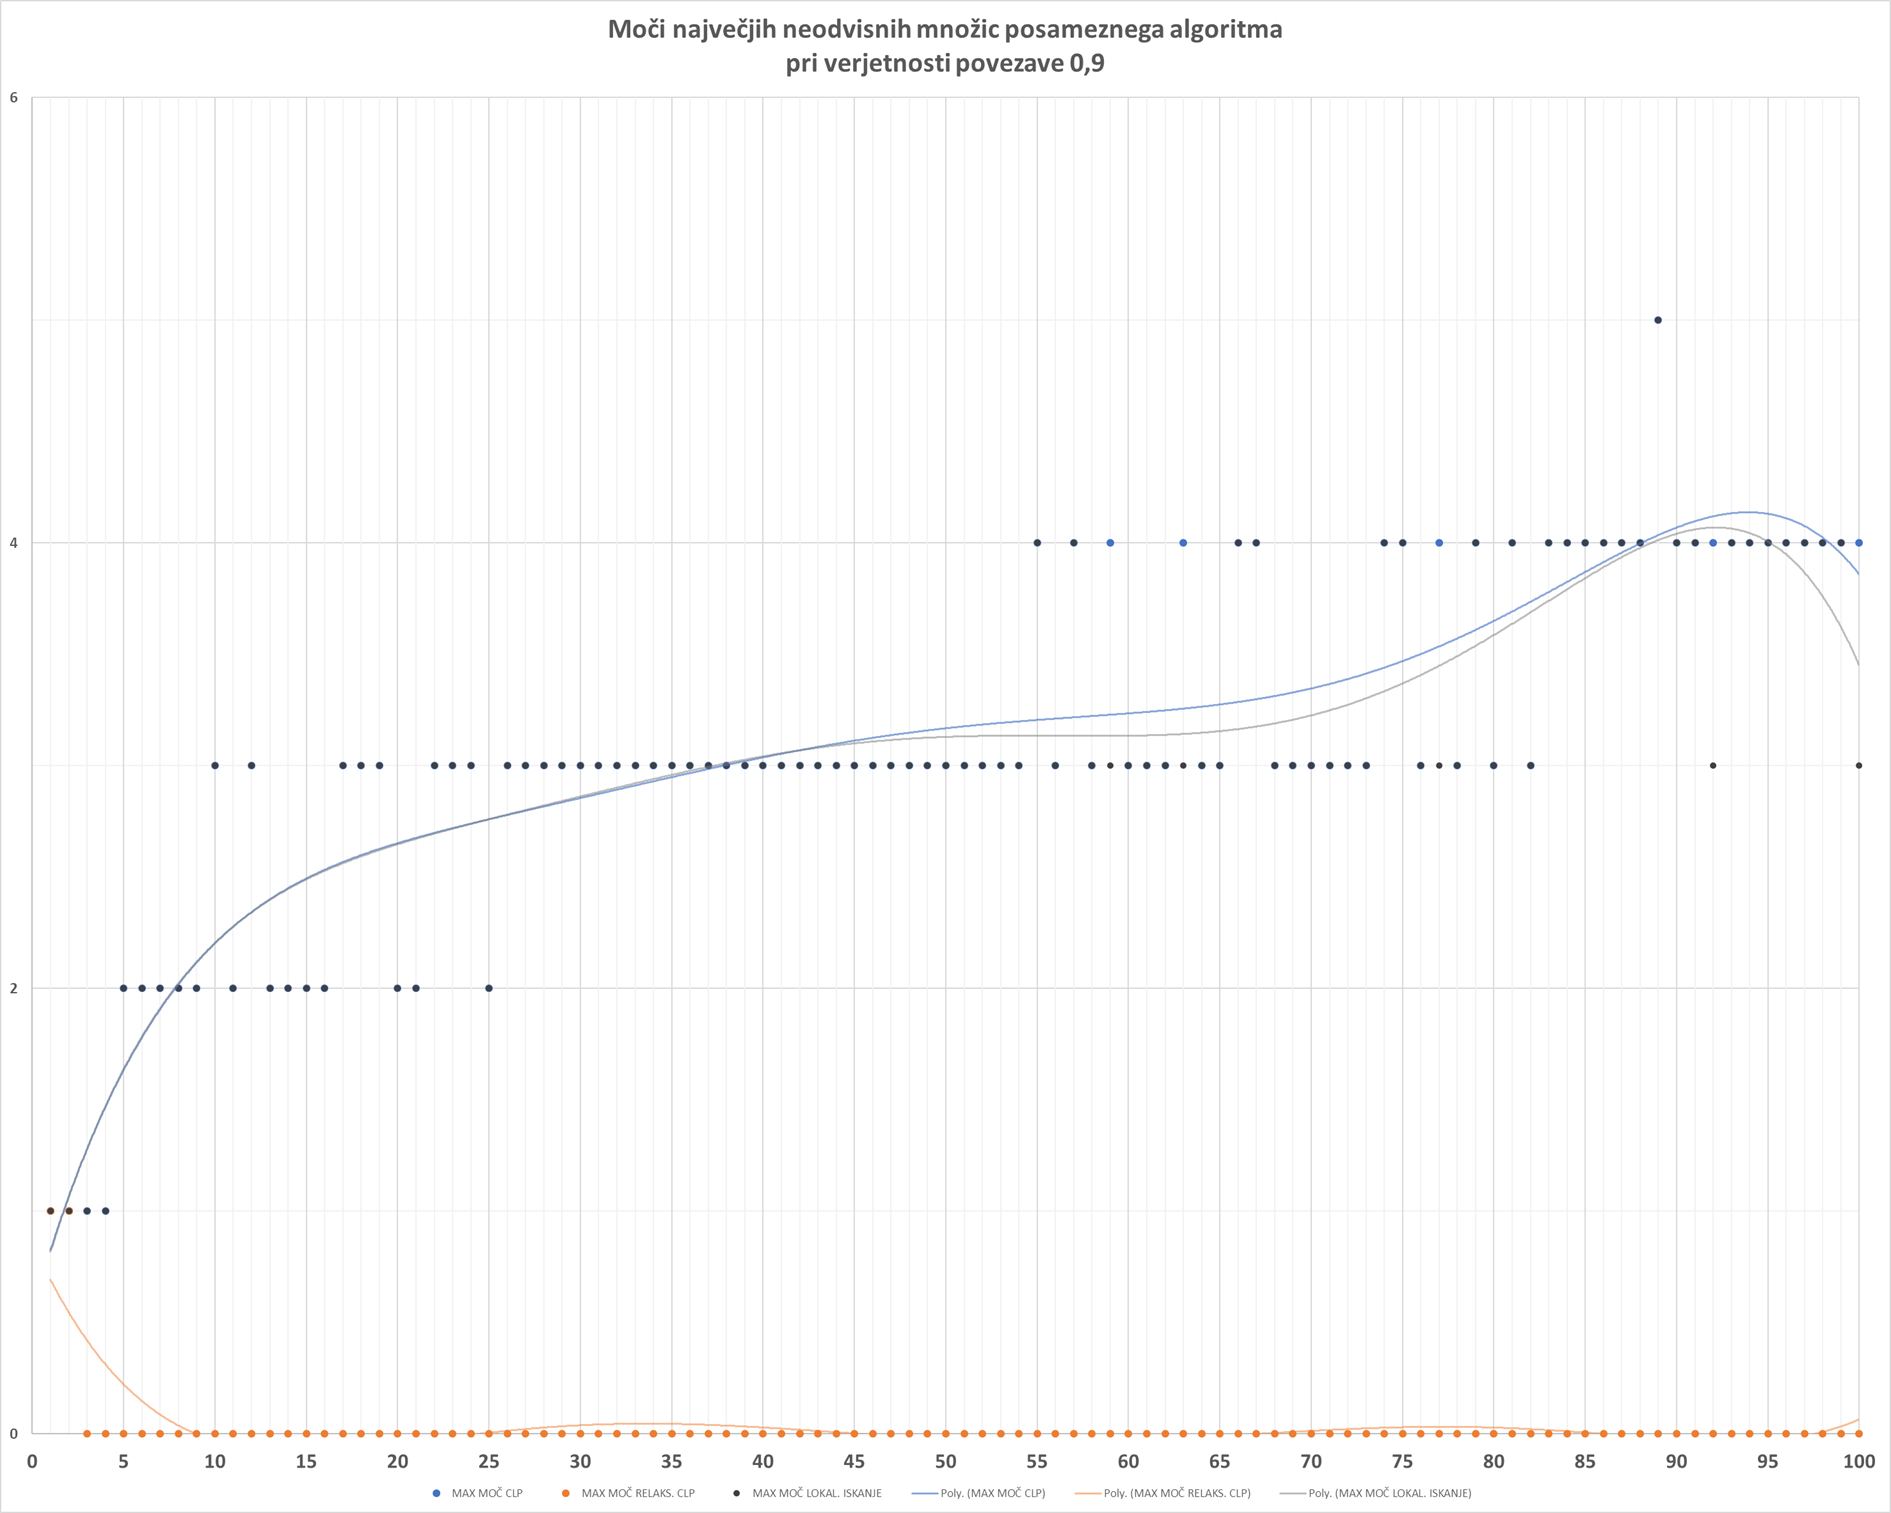
\includegraphics[scale=0.28]{./Slike/0,9 moci.png}
  \caption{Moči največjih neodvisnih množic pri verjetnosti povezave 0,9}
  \label{fig:moc0,9} 
\end{figure}

\subsubsection{Časovna zahtevnost na naključnih grafih} % ============================================
Pri analizi časovne zahtevnosti sem se omejil zgolj na algoritem za lokalno iskanje. Časovne zahtevnosti CLP nisem meril, saj je izjemno neučinkovit,  prav tako ne relaksacije CLP, saj nam za velike grafe skoraj vedno vrača prazno množico.

V namen analize časovne zahtevnosti algoritma lokalnega iskanja sem na grafu z verjetnostjo povezave dveh vozlišč 0,3 in 50 ponovitvami zunanje zanke izvedel algoritem. Neodvisna spremenljivka je bila torej število vozlišč, ki sem jo povečeval s korakom 50 do končne velikosti grafa z 2451 vozlišči. Meritve časa sem izvedel trikrat in nato vzel povprečje vseh treh časov pri posamezni velikosti grafa. Na grafu je prikazan tudi aproksimacijski polinom šeste stopnje in napoved za povečevanje časovne zahtevnosti za grafe do velikosti 3000 vozlišč.


\begin{figure}[H]
\centering
  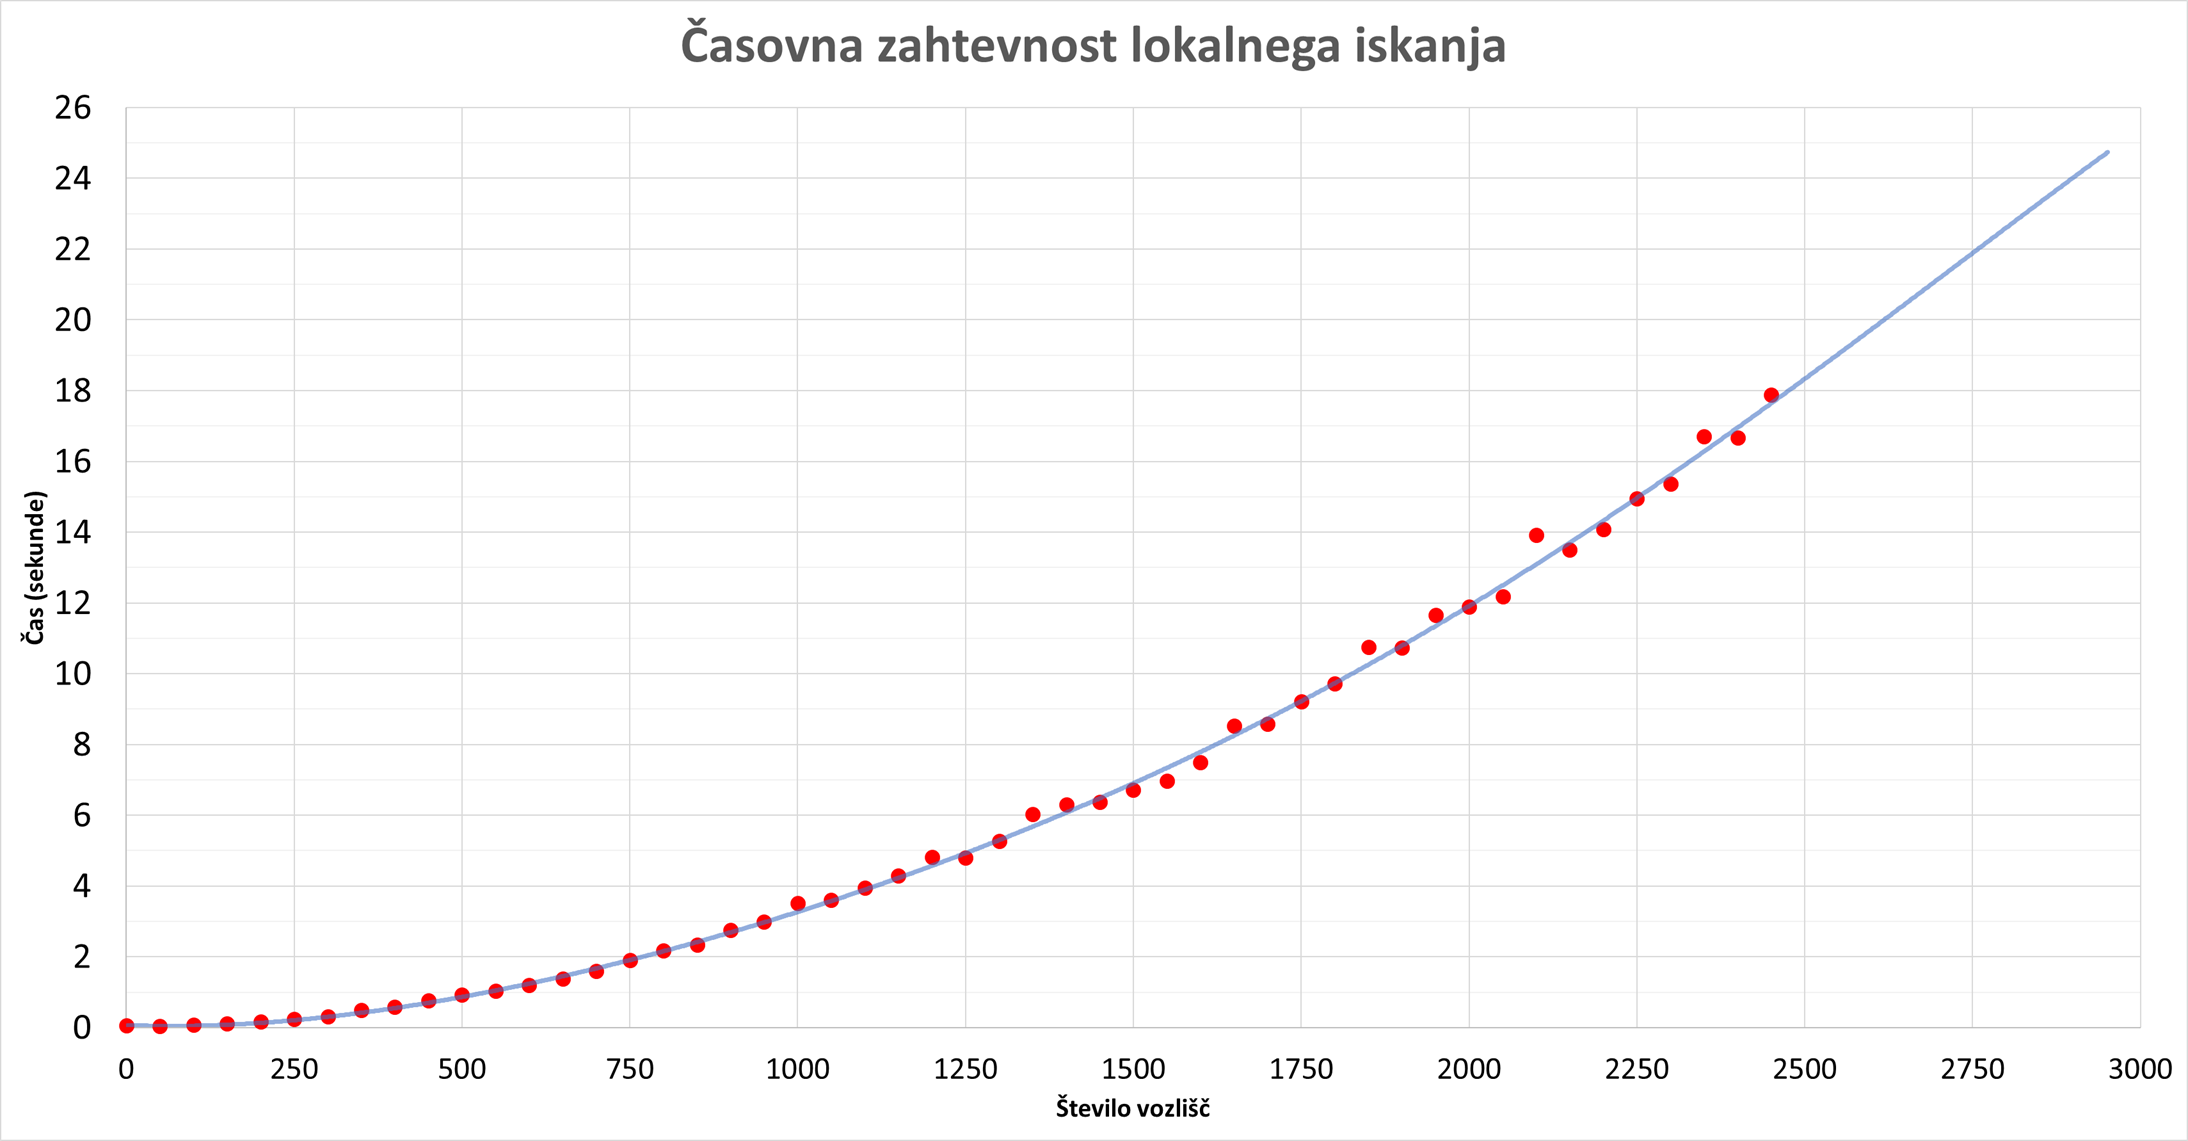
\includegraphics[scale=0.29]{./Slike/casovna_ zahtevnost_LOKISK.png}
  \caption{Časovna zahtevnost lokalnega iskanja}
  \label{fig:casovna zahtevnost} 
\end{figure}


\subsection{Analiza algoritmov na Petersenovem grafu}
V nadaljevanju sem izvedel tudi algeoritme na Petersenovem grafu. To je graf z 10 točkami in 15 povezavami. Stopnja vsake točke Petersenovega grafa je enaka 3.


\begin{figure}[H]
\centering
  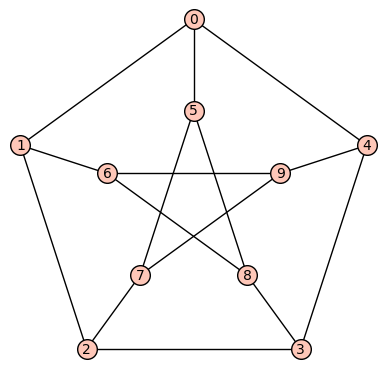
\includegraphics[scale=0.35]{./Slike/Petersenov graf.png}
  \caption{Petersenov graf}
\end{figure}

CLP in lokalno iskanje vedno najdeta enako moč največje neodvisne množice, medtem ko so vozlišča v njej enaka le v 10 odstotkih poskusov. Relaksacija CLP pa vedno vrača prazno množico. Časovne zahtevnosti in moči množice $I$ so podane v spodnji tabeli.

\begin{table}[H]
\centering
\begin{tabular}{|p{3cm}||p{3.2cm}|p{4.7cm}|}
\hline
\textbf{Algoritem}  & \textbf{Moč množice $I$} & \textbf{Čas izvedbe algoritma} \\ \hline
CLP    & 4 &  		   0.0106859 $s$\\ \hline
Relaks. CLP    & 0  &  0.0023558 $s$   \\ \hline
Lokalno iskanje & 4 &  0.0069702 $s$ \\ \hline
\end{tabular}
\caption{Moč množice I in časovna zahtevnost iskanja na Petersenovem grafu}
\label{fig:petersenov} 
\end{table}

\subsection{Analiza algoritmov na hiperkockah}
Pri analizi vseh treh algoritmov na hiperkockah sem pogledal največje množice neodvisnih vozlišč grafa in časovne zahtevnosti algoritmov na hiperkockah na 4, 8, 16, 32, 64 in 128 vozliščih. 

\begin{figure}[H]
\centering
  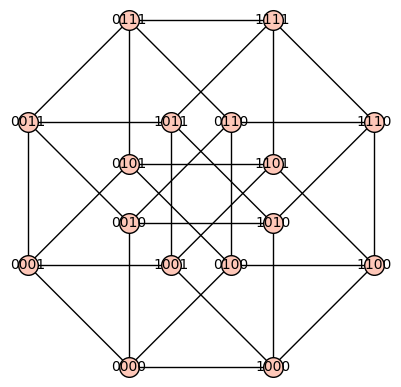
\includegraphics[scale=0.40]{./Slike/Cube graph 4.png}
  \caption{Hiperkocka na 16 vozliščih}
\end{figure}

\begin{table}[H]
\centering
\begin{tabular}{|p{3cm}||p{1cm}|p{2.7cm}|p{3.2cm}|}
\hline
\textbf{Število vozlišč}  & \textbf{CLP} & \textbf{Relaks. CLP} & \textbf{Lokalno iskanje} \\ \hline
\textbf{4}     & 2 &2  &2  \\ \hline
\textbf{8}    & 4 & 4 &4  \\ \hline
\textbf{16}   & 8 & 8  &8  \\ \hline
\textbf{32}  & 16 &16  &16  \\ \hline
\textbf{64}   & 32 & 32 &  32 \\ \hline
\textbf{128} & 64 & 64 & 64  \\ \hline
\end{tabular}
\caption{Moč množice $I$ na hiperkockah}
\label{fig:hipekocka I} 
\end{table}
Vidimo, da so vse tri množice $I$ ves čas enake in je njihova moč enaka ravno polovici števila vseh vozlišč grafa. To je seveda logično, saj gre za dvodelen graf. 

\newpage
\subsubsection{Časovna zahtevnost algoritmov na hiperkockah}
Analiziral sem tudi časovno zahtevnost algoritmov na hiperkockah velikosti z 4 do 2048 vozlišči.
V spodnji tabeli so prikazane časovne zahtevnosti do 128 vozlišč, v nadalnjem grafu pa so grafično prikazani še vsi rezultati.

\begin{table}[H]
\centering
\begin{tabular}{|p{3cm}||p{2.8cm}|p{2.8cm}|p{3.2cm}|}
\hline
\textbf{Število vozlišč}  & \textbf{CLP} & \textbf{Relaks. CLP} & \textbf{Lokalno iskanje} \\ \hline
\textbf{4}&	0.0027&	0.0011	&0.0033\\ \hline
\textbf{8}&	0.0027	&0.0036	&0.0053\\ \hline
\textbf{16}&0.0056	&0.0034	&0.0386\\ \hline
\textbf{32}&0.0100&	0.0280	&0.0239\\ \hline
\textbf{64}&0.0180	&0.0160	&0.0270\\ \hline
\textbf{128}&0.0275	&0.0440	&0.0392\\ \hline
\end{tabular}
\caption{Časovna zahtevnost algoritmov na hiperkockah (v sekundah)}
\label{fig:hipekocka I} 
\end{table}


\begin{figure}[H]
\centering
  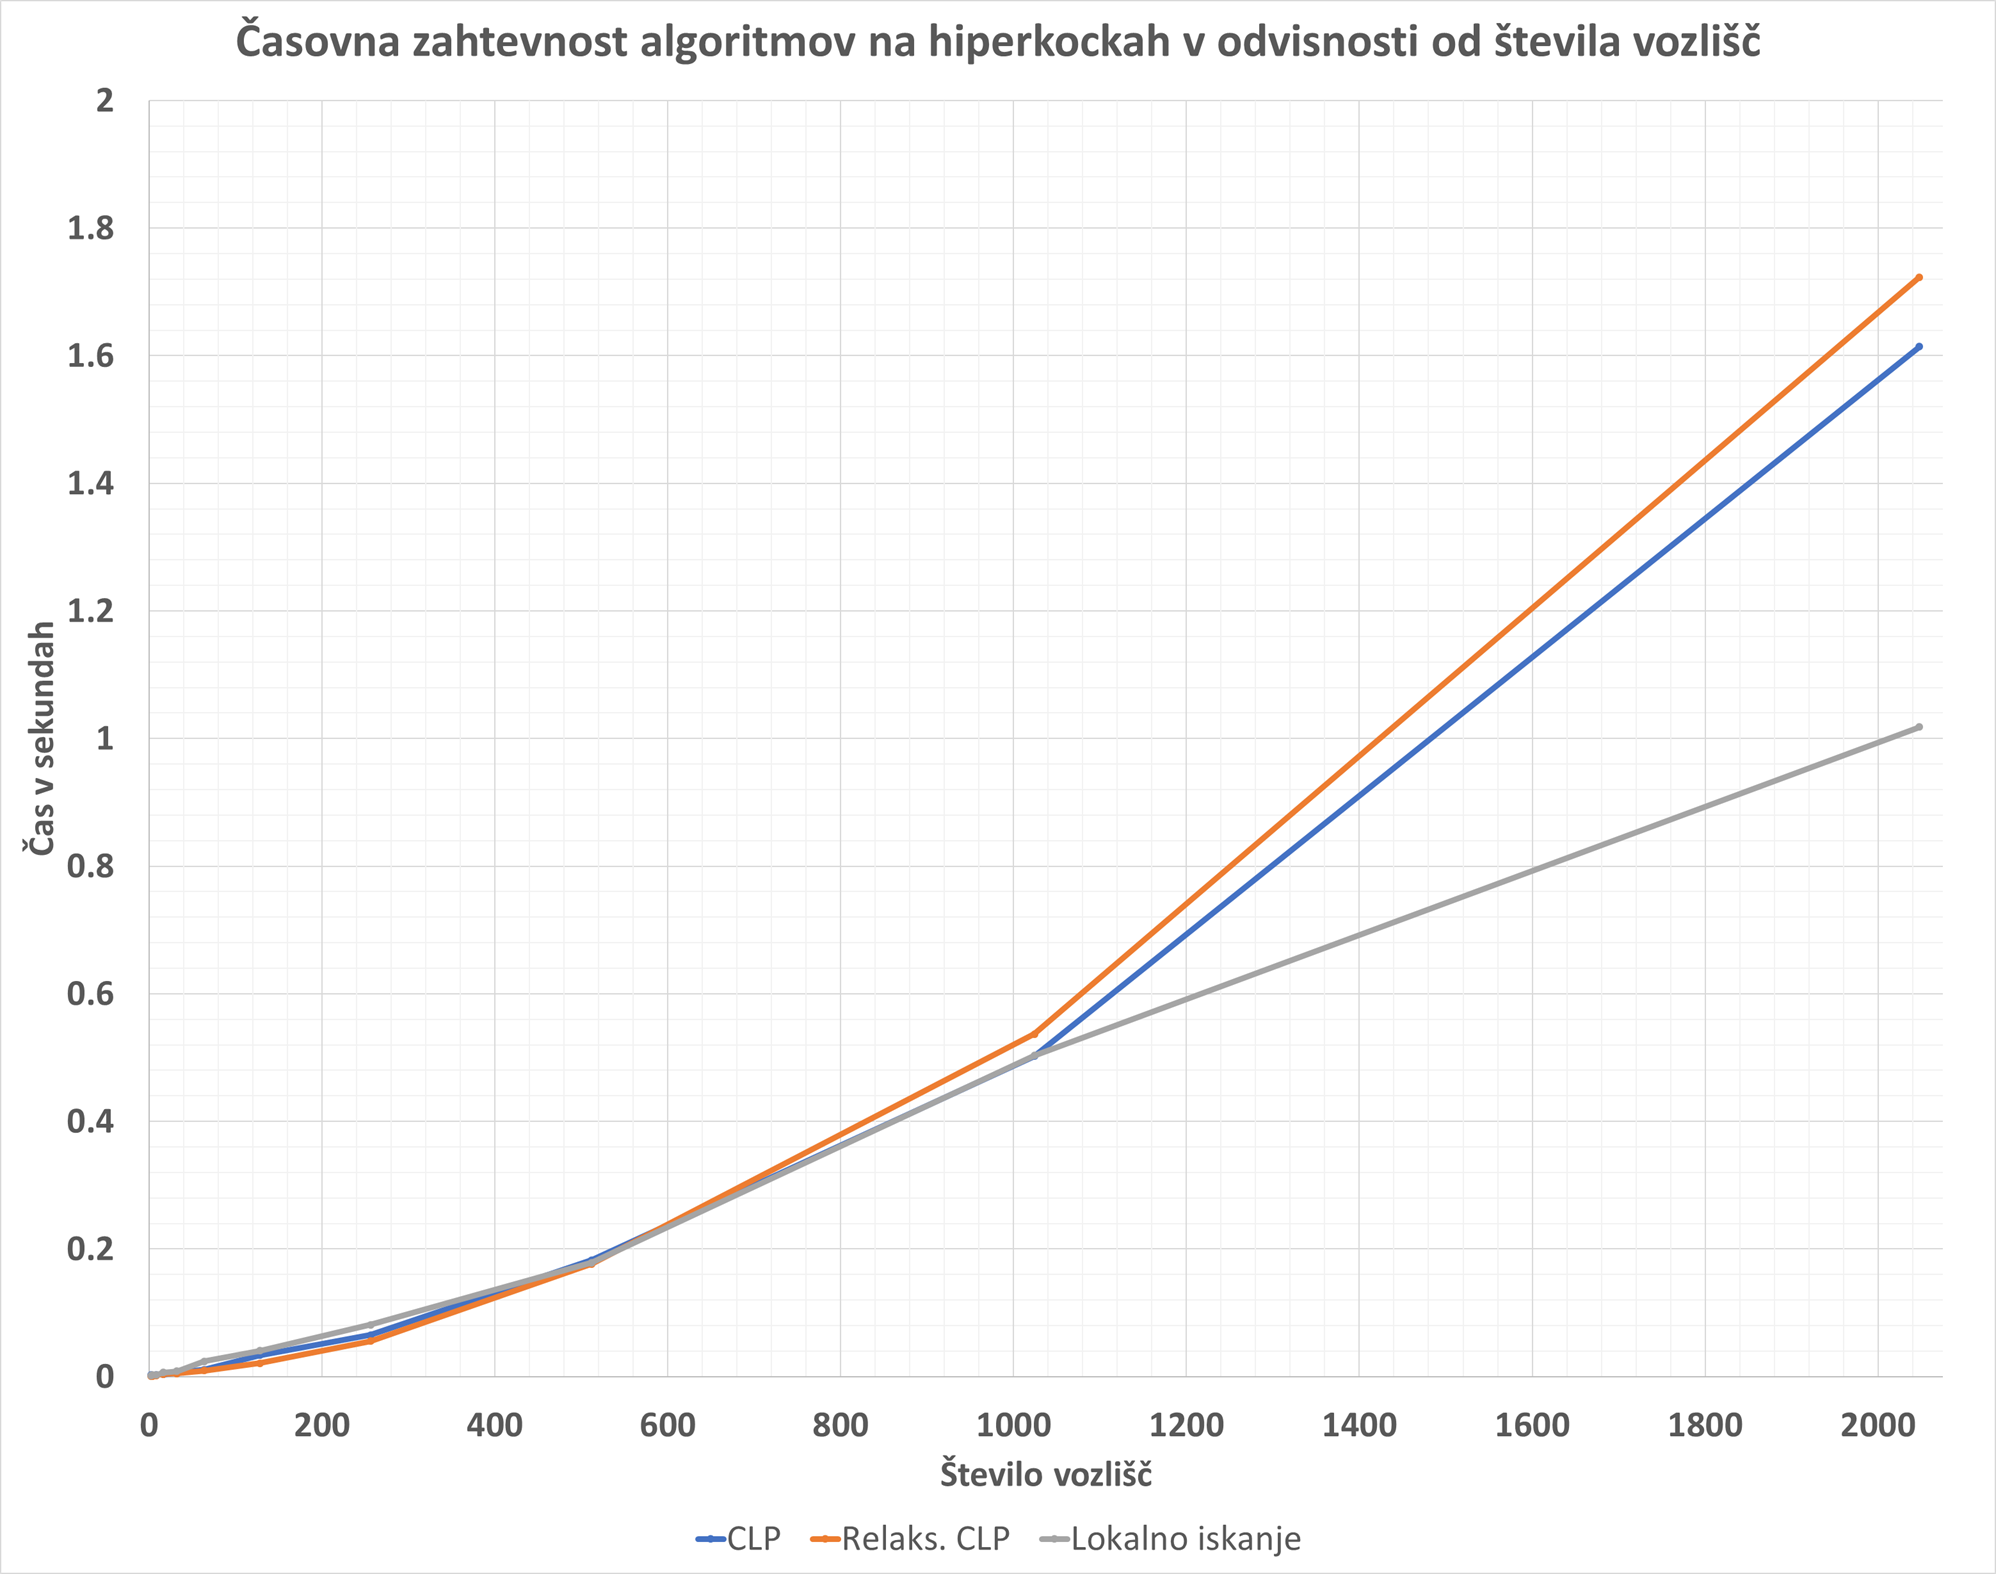
\includegraphics[scale=0.30]{./Slike/Casovna_zahtevnost_hiperkocke.png}
  \caption{Časovna zahtevnost na hiperkockah}
\end{figure}

\section{Zaključek}
Generalno gledano za vse rezultate testiranj torej velja, da je moč množice dobljene s CLP vedno večja ali enaka moči množice dobljene z lokalnim iskanjem. Na naključnih grafih in pri Petersenovem grafu je relaksacija CLP praktično neuporabna, saj prepogosto vrača prazne množice, kar pomeni, da je očitno optimalna vrednost kriterijske funkcije, ko imajo vsa vozlišča vrednost $x_v$ enako $\frac{1}{2}$. Zanimivo je, da z večanjem verjetnosti, moč največje neodvisne množice CLP in lokalnega iskanja postaja konstantna na določenih intervalih števila vozlišč. Z večanjem števila vozlišč, se moč množice tudi precej počasneje povečuje in pri zelo povezanih grafih nikoli celo ne preseže vrednosti 5.

Na Petersonovem grafu pričakovano CLP in lokalno iskanje vračata optimalen rezultat, relaksacija CLP pa ponovno odpove in vrača prazno množico. Tudi v tem primeru je lokalno iskanje izrazito hitrejše od algoritma CLP.

Pri hiperkockah pa zaradi dvodelnosti grafa vsi trije algoritmi vračajo enako optimalno množico, ki je seveda enaka ravno polovici moči množice vozlišč. Tudi tu je časovna zahtevnost lokalnega iskanja najmanjša. Vidimo, da se do 1000 vozlišč časi ne razlikujejo prav dosti, nato pa začne prihajati do večjih razlik.\\

Priporočil bi uporabo algoritma lokalnega iskanja, saj je precej hitrejši kot CLP. Hkrati pa je tudi CLP uporaben za preproste analize na manjših grafih. Nasprotno pa bi uporabo relaksacije CLP odvsetoval, saj prepogosto prihaja do optimalne rešitve, ko imajo vsa ogljišča vrednost $\frac{1}{2}$ in nam zato njegov rezultat ne pove prav dosti.


% ==========================================================
\end{document}